\chapter{L12 -- Sottospazio di raggiungibilità e forma standard di raggiungibilità}

\section{Idea della lezione}

In questa lezione vogliamo rispondere a una domanda strutturale molto importante:

\begin{quote}
\emph{È possibile riscrivere il sistema separando chiaramente la parte raggiungibile da quella non raggiungibile?}
\end{quote}

La risposta è sì.  
Il punto di partenza è capire bene che lo \textbf{spazio di raggiungibilità} non è solo l’insieme degli stati che si possono raggiungere con un opportuno ingresso, ma è anche un sottospazio con una struttura molto precisa: è un sottospazio \textbf{\(A\)-invariante} che contiene l’immagine di \(B\).

Questa proprietà permette di scegliere un cambio di coordinate adatto, con cui il sistema assume una forma a blocchi nella quale:
\begin{itemize}
    \item una parte dello stato è effettivamente influenzabile dall’ingresso;
    \item l’altra parte evolve da sola, senza poter essere modificata dal controllo.
\end{itemize}

Questa è la cosiddetta \textbf{forma standard di raggiungibilità}.

\section{Richiamo: spazio di raggiungibilità}

Consideriamo un sistema lineare stazionario.

Nel caso tempo continuo:
\begin{equation}
\dot x(t)=Ax(t)+Bu(t),
\qquad x(t)\in\R^n,\quad u(t)\in\R^m.
\end{equation}

Nel caso tempo discreto:
\begin{equation}
x(k+1)=Ax(k)+Bu(k),
\qquad x(k)\in\R^n,\quad u(k)\in\R^m.
\end{equation}

La matrice di raggiungibilità associata alla coppia \((A,B)\) è
\begin{equation}
R=\begin{bmatrix}
B & AB & A^2B & \cdots & A^{n-1}B
\end{bmatrix}.
\end{equation}

Lo \textbf{spazio di raggiungibilità} è definito come
\begin{equation}
\mathcal{R}=\operatorname{Im}(R).
\end{equation}

Nel discreto, se si vuole enfatizzare il numero di passi, si considera anche
\begin{equation}
R_t=\begin{bmatrix}
B & AB & \cdots & A^{t-1}B
\end{bmatrix},
\qquad
\mathcal{R}_t=\operatorname{Im}(R_t).
\end{equation}

Il significato è il seguente:
\begin{itemize}
    \item \(\mathcal{R}_t\) contiene gli stati raggiungibili dall’origine in \(t\) passi;
    \item \(\mathcal{R}\) contiene tutti gli stati raggiungibili dall’origine e coincide con il sottospazio generato dagli effetti successivi di \(B,AB,\dots,A^{n-1}B\).
\end{itemize}

\section{Teorema fondamentale sul sottospazio di raggiungibilità}

\begin{teorema}
Lo spazio di raggiungibilità
\[
\mathcal{R}=\operatorname{Im}(R)
\]
è il più piccolo sottospazio \(A\)-invariante che contiene \(\operatorname{Im}(B)\).
\end{teorema}

Questo teorema è fondamentale, perché caratterizza \(\mathcal{R}\) non solo come insieme di stati ottenibili con un ingresso, ma come oggetto geometrico ben preciso.

\subsection{Dimostrazione}

Dimostriamo il risultato in tre passaggi.

\subsubsection*{1. \(\mathcal{R}\) contiene \(\operatorname{Im}(B)\)}

Per definizione,
\[
R=\begin{bmatrix}
B & AB & A^2B & \cdots & A^{n-1}B
\end{bmatrix}.
\]
Le colonne di \(B\) sono tra le colonne di \(R\), quindi ogni vettore di \(\operatorname{Im}(B)\) appartiene a \(\operatorname{Im}(R)\). Dunque
\[
\operatorname{Im}(B)\subseteq \mathcal{R}.
\]

\subsubsection*{2. \(\mathcal{R}\) è \(A\)-invariante}

Prendiamo un qualunque vettore \(x\in\mathcal{R}\).  
Allora esiste \(y\) tale che
\[
x=Ry.
\]
Moltiplicando per \(A\),
\[
Ax=A(Ry)=
\begin{bmatrix}
AB & A^2B & \cdots & A^nB
\end{bmatrix}y.
\]

Il problema apparente è il termine \(A^nB\), che non compare esplicitamente in \(R\).  
Però, per il teorema di Cayley--Hamilton, \(A^n\) si può esprimere come combinazione lineare di \(I,A,\dots,A^{n-1}\). Quindi anche \(A^nB\) è combinazione lineare di
\[
B,\,AB,\,A^2B,\dots,A^{n-1}B.
\]
Ne segue che \(Ax\) è ancora combinazione lineare delle colonne di \(R\), cioè
\[
Ax\in\operatorname{Im}(R)=\mathcal{R}.
\]
Pertanto \(\mathcal{R}\) è \(A\)-invariante.

\subsubsection*{3. \(\mathcal{R}\) è il più piccolo tra questi sottospazi}

Sia \(S\subseteq\R^n\) un sottospazio \(A\)-invariante tale che
\[
\operatorname{Im}(B)\subseteq S.
\]
Poiché \(S\) contiene \(\operatorname{Im}(B)\), contiene le colonne di \(B\).  
Essendo \(S\) \(A\)-invariante, contiene anche le colonne di \(AB\), poi di \(A^2B\), e così via. Per induzione,
\[
\operatorname{Im}(A^kB)\subseteq S
\qquad \forall k=0,1,\dots,n-1.
\]
Quindi tutte le colonne di \(R\) appartengono a \(S\), e dunque
\[
\mathcal{R}=\operatorname{Im}(R)\subseteq S.
\]

Abbiamo quindi dimostrato che \(\mathcal{R}\) è il più piccolo sottospazio \(A\)-invariante che contiene \(\operatorname{Im}(B)\).
\qed

\section{Interpretazione geometrica}

Il significato intuitivo del teorema è molto chiaro:

\begin{itemize}
    \item l’ingresso entra nel sistema attraverso \(B\), quindi inizialmente può generare solo vettori in \(\operatorname{Im}(B)\);
    \item poi la dinamica libera \(A\) prende quei vettori e li evolve nel tempo;
    \item quindi lo spazio effettivamente esplorabile dall’ingresso è il più piccolo sottospazio che contiene \(\operatorname{Im}(B)\) e che sia chiuso rispetto all’azione di \(A\).
\end{itemize}

Possiamo visualizzarlo così.

\begin{figure}[H]
\centering
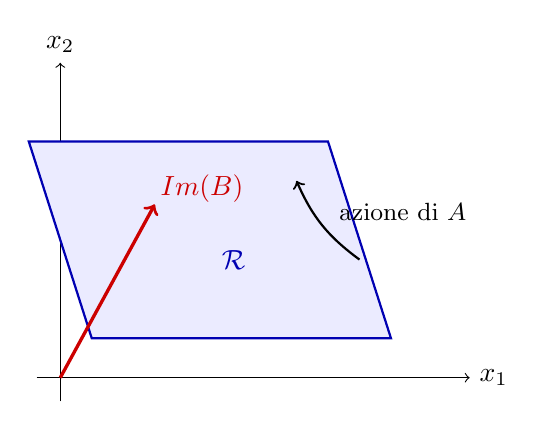
\begin{tikzpicture}[scale=1]
    % assi
    \draw[->] (-0.3,0) -- (5.2,0) node[right] {$x_1$};
    \draw[->] (0,-0.3) -- (0,4.0) node[above] {$x_2$};

    % parallelogramma dello spazio raggiungibile
    \fill[blue!8] (0.4,0.5) -- (4.2,0.5) -- (3.4,3.0) -- (-0.4,3.0) -- cycle;
    \draw[blue!70!black, thick] (0.4,0.5) -- (4.2,0.5) -- (3.4,3.0) -- (-0.4,3.0) -- cycle;

    % immagine di B
    \draw[red!80!black, very thick, ->] (0,0) -- (1.2,2.2);
    \node[red!80!black] at (1.8,2.4) {$\operatorname{Im}(B)$};

    % label R
    \node[blue!70!black] at (2.2,1.5) {$\mathcal{R}$};

    % freccia dinamica A
    \draw[->, thick] (3.8,1.5) to[bend left=15] (3.0,2.5);
    \node at (4.35,2.1) {\small azione di \(A\)};
\end{tikzpicture}
\caption{Interpretazione geometrica dello spazio di raggiungibilità.}
\end{figure}

\section{Invarianza rispetto al cambio di coordinate}

La raggiungibilità è una proprietà strutturale della coppia \((A,B)\), quindi non dipende dal sistema di coordinate usato per descrivere lo stato.

Consideriamo un cambio di coordinate invertibile
\begin{equation}
x=Tz,
\qquad T\in\R^{n\times n}\ \text{invertibile}.
\end{equation}

Nel discreto:
\[
x^{+}=Ax+Bu
\quad \Longrightarrow \quad
Tz^{+}=ATz+Bu.
\]
Moltiplicando per \(T^{-1}\),
\[
z^{+}=T^{-1}AT\,z+T^{-1}Bu.
\]
Quindi il sistema trasformato è
\begin{equation}
z^{+}=\tilde A z+\tilde B u,
\qquad
\tilde A=T^{-1}AT,\qquad \tilde B=T^{-1}B.
\end{equation}

La matrice di raggiungibilità nelle nuove coordinate è
\[
R_z=
\begin{bmatrix}
\tilde B & \tilde A\tilde B & \cdots & \tilde A^{n-1}\tilde B
\end{bmatrix}.
\]
Sostituendo,
\[
R_z=
\begin{bmatrix}
T^{-1}B & T^{-1}AB & \cdots & T^{-1}A^{n-1}B
\end{bmatrix}
= T^{-1}R.
\]

Poiché \(T^{-1}\) è invertibile,
\[
\rank(R_z)=\rank(R).
\]
Quindi la dimensione dello spazio di raggiungibilità non cambia.

\begin{osservazione}
La raggiungibilità è una proprietà del sistema, non della rappresentazione scelta.  
Questo è il motivo per cui ha senso cercare un cambio di coordinate che renda la struttura del sistema più trasparente.
\end{osservazione}

\section{Separazione tra parte raggiungibile e non raggiungibile}

Sia
\[
r=\dim(\mathcal{R})=\rank(R).
\]
Se \(r<n\), il sistema non è completamente raggiungibile.

In questo caso scegliamo:
\begin{itemize}
    \item una matrice \(T_R\in\R^{n\times r}\) le cui colonne formino una base di \(\mathcal{R}\);
    \item una matrice \(T_N\in\R^{n\times(n-r)}\) che completi tale base a una base di tutto \(\R^n\).
\end{itemize}

Definiamo allora
\begin{equation}
T=\begin{bmatrix}
T_R & T_N
\end{bmatrix}.
\end{equation}
Essendo le colonne di \(T\) una base di \(\R^n\), la matrice \(T\) è invertibile.

Passando alle nuove coordinate \(x=Tz\), possiamo scrivere
\[
z=
\begin{pmatrix}
z_R\\
z_N
\end{pmatrix},
\]
dove:
\begin{itemize}
    \item \(z_R\in\R^r\) rappresenta la parte raggiungibile;
    \item \(z_N\in\R^{n-r}\) rappresenta la parte non raggiungibile.
\end{itemize}

\section{Forma a blocchi della dinamica}

Poiché \(\mathcal{R}\) è \(A\)-invariante, se uno stato appartiene a \(\mathcal{R}\), allora anche la sua evoluzione libera appartiene a \(\mathcal{R}\).

Nelle nuove coordinate, i vettori di \(\mathcal{R}\) hanno la forma
\[
z=
\begin{pmatrix}
z_R\\
0
\end{pmatrix}.
\]

Scriviamo allora la matrice trasformata \(\tilde A=T^{-1}AT\) in forma a blocchi:
\begin{equation}
\tilde A=
\begin{bmatrix}
A_R & A_{RN}\\
A_{NR} & A_N
\end{bmatrix}.
\end{equation}

Applicandola a un vettore della forma \(\begin{pmatrix} z_R \\ 0 \end{pmatrix}\), otteniamo
\[
\tilde A
\begin{pmatrix}
z_R\\
0
\end{pmatrix}
=
\begin{pmatrix}
A_R z_R\\
A_{NR} z_R
\end{pmatrix}.
\]
Ma questo vettore deve appartenere ancora a \(\mathcal{R}\), quindi la sua parte inferiore deve essere nulla per ogni \(z_R\). Ne segue
\[
A_{NR}=0.
\]

Dunque la matrice assume necessariamente la forma
\begin{equation}
\tilde A=
\begin{bmatrix}
A_R & A_{RN}\\
0 & A_N
\end{bmatrix}.
\label{eq:L12_Atriangolare}
\end{equation}

\section{Forma di \(\tilde B\)}

Poiché \(\operatorname{Im}(B)\subseteq\mathcal{R}\), nelle coordinate adattate alla decomposizione dello spazio di stato il vettore \(Bu\) deve avere componenti solo nella parte raggiungibile.

Di conseguenza
\begin{equation}
\tilde B=T^{-1}B=
\begin{pmatrix}
B_R\\
0
\end{pmatrix}.
\label{eq:L12_Btriangolare}
\end{equation}

\section{Forma standard di raggiungibilità}

Abbiamo così ottenuto la \textbf{forma standard di raggiungibilità}.

Nel discreto:
\begin{equation}
z^{+}=
\begin{bmatrix}
A_R & A_{RN}\\
0 & A_N
\end{bmatrix}
z+
\begin{pmatrix}
B_R\\
0
\end{pmatrix}u.
\label{eq:L12_formastandard_td}
\end{equation}

Nel continuo:
\begin{equation}
\dot z=
\begin{bmatrix}
A_R & A_{RN}\\
0 & A_N
\end{bmatrix}
z+
\begin{pmatrix}
B_R\\
0
\end{pmatrix}u.
\label{eq:L12_formastandard_tc}
\end{equation}

\subsection*{Interpretazione}

Questa forma dice esattamente che:
\begin{itemize}
    \item il sottosistema \(z_R\) è la parte raggiungibile;
    \item il sottosistema \(z_N\) è la parte non raggiungibile;
    \item l’ingresso agisce solo sul primo blocco.
\end{itemize}

Più precisamente, la dinamica è
\[
\begin{cases}
z_R^{+}=A_R z_R + A_{RN} z_N + B_R u,\\
z_N^{+}=A_N z_N.
\end{cases}
\]
Quindi la parte non raggiungibile evolve in modo autonomo.

\begin{figure}[H]
\centering
\begin{tikzpicture}[>=Latex, node distance=2.8cm]
    \node[draw, rounded corners, minimum width=3.2cm, minimum height=1.2cm, fill=blue!8] (zr) {$z_R$};
    \node[draw, rounded corners, minimum width=3.2cm, minimum height=1.2cm, fill=gray!10, right of=zr] (zn) {$z_N$};

    \draw[->, thick] (-2.2,0) -- (zr.west) node[midway, above] {$u$};
    \draw[loop above, thick] (zr) to node[above] {$A_R$} (zr);
    \draw[loop above, thick] (zn) to node[above] {$A_N$} (zn);
    \draw[->, thick] (zr.east) -- (zn.west) node[midway, above] {$A_{RN}$};

    \node[below=0.7cm of zr] {\small sottosistema raggiungibile};
    \node[below=0.7cm of zn] {\small sottosistema non raggiungibile};
\end{tikzpicture}
\caption{Interpretazione della forma standard di raggiungibilità.}
\end{figure}

\section{Sottosistema raggiungibile e sottosistema non raggiungibile}

La decomposizione precedente ha un significato molto importante.

\subsection*{Parte raggiungibile}

Il blocco \((A_R,B_R)\) rappresenta il sottosistema su cui l’ingresso può effettivamente agire.  
Infatti in quella dinamica compare il termine \(B_Ru\).

\subsection*{Parte non raggiungibile}

Il blocco \(A_N\) rappresenta invece il sottosistema che evolve in modo completamente autonomo:
\[
z_N^{+}=A_N z_N.
\]
Qui il controllo non compare né direttamente né indirettamente.

Questo è il contenuto matematico preciso della frase:
\begin{quote}
\emph{La parte non raggiungibile evolve in anello aperto.}
\end{quote}

\subsection*{Conclusione importante}

Sul sottosistema raggiungibile posso provare a fare quello che voglio.  
Sul sottosistema non raggiungibile, invece, con l’ingresso non posso fare assolutamente nulla.

\section{Il sottosistema raggiungibile è completamente raggiungibile}

Una volta portato il sistema nella forma standard di raggiungibilità, la coppia \((A_R,B_R)\) risulta completamente raggiungibile.

Il motivo è concettualmente semplice: se il blocco raggiungibile non fosse completamente raggiungibile, allora al suo interno esisterebbe ancora una parte non raggiungibile. Ma questo contraddirebbe il fatto di aver già isolato tutta la parte raggiungibile nel primo blocco.

In altre parole, la decomposizione è costruita proprio in modo da raccogliere tutta la dinamica raggiungibile nel blocco \(A_R\).

\section{Autovalori raggiungibili e autovalori non raggiungibili}

Poiché \(\tilde A\) è triangolare a blocchi,
\[
\tilde A=
\begin{bmatrix}
A_R & A_{RN}\\
0 & A_N
\end{bmatrix},
\]
i suoi autovalori sono l’unione degli autovalori dei blocchi diagonali:
\[
\sigma(\tilde A)=\sigma(A_R)\cup\sigma(A_N).
\]

Da qui nasce la terminologia:
\begin{itemize}
    \item gli autovalori di \(A_R\) si chiamano \textbf{autovalori raggiungibili};
    \item gli autovalori di \(A_N\) si chiamano \textbf{autovalori non raggiungibili}.
\end{itemize}

Questa distinzione è fondamentale in controllo, perché:
\begin{quote}
\emph{gli autovalori non raggiungibili non possono essere modificati tramite l’ingresso.}
\end{quote}

\section{Effetto sulla funzione di trasferimento}

Consideriamo ora il sistema trasformato, nel caso continuo:
\[
\dot z=
\begin{bmatrix}
A_R & A_{RN}\\
0 & A_N
\end{bmatrix}z+
\begin{pmatrix}
B_R\\
0
\end{pmatrix}u,
\qquad
y=
\begin{bmatrix}
C_R & C_N
\end{bmatrix}z+Du.
\]

La funzione di trasferimento vale
\[
G(s)=C(sI-A)^{-1}B+D.
\]
Passando alle coordinate trasformate,
\[
G(s)=\tilde C(sI-\tilde A)^{-1}\tilde B + D.
\]

Ora
\[
sI-\tilde A=
\begin{bmatrix}
sI_r-A_R & -A_{RN}\\
0 & sI_{n-r}-A_N
\end{bmatrix},
\]
che è una matrice triangolare a blocchi. La sua inversa ha quindi la forma
\[
(sI-\tilde A)^{-1}=
\begin{bmatrix}
(sI_r-A_R)^{-1} & *\\
0 & (sI_{n-r}-A_N)^{-1}
\end{bmatrix}.
\]

Moltiplicando per \(\tilde B\),
\[
(sI-\tilde A)^{-1}\tilde B=
\begin{pmatrix}
(sI_r-A_R)^{-1}B_R\\
0
\end{pmatrix}.
\]
Infine
\begin{align}
G(s)
&=
\begin{bmatrix}
C_R & C_N
\end{bmatrix}
\begin{pmatrix}
(sI_r-A_R)^{-1}B_R\\
0
\end{pmatrix}+D\\
&=
C_R(sI_r-A_R)^{-1}B_R+D.
\end{align}

\begin{osservazione}
La funzione di trasferimento dipende solo dal sottosistema raggiungibile.  
La parte non raggiungibile non compare nella dinamica ingresso--uscita.
\end{osservazione}

Questa osservazione è molto importante: se una dinamica interna non è raggiungibile, non la si vede pilotando il sistema tramite l’ingresso.

\section{Esempio}

Consideriamo il sistema
\[
A=
\begin{bmatrix}
1 & 0 & 0\\
1 & 2 & 1\\
0 & 1 & -2
\end{bmatrix},
\qquad
B=
\begin{bmatrix}
0\\
1\\
0
\end{bmatrix},
\qquad
C=
\begin{bmatrix}
0 & 0 & 1
\end{bmatrix}.
\]

\subsection*{1. Calcolo della matrice di raggiungibilità}

Calcoliamo:
\[
AB=
\begin{bmatrix}
0\\
2\\
1
\end{bmatrix},
\qquad
A^2B=A(AB)=
\begin{bmatrix}
0\\
5\\
0
\end{bmatrix}.
\]
Quindi
\[
R=
\begin{bmatrix}
B & AB & A^2B
\end{bmatrix}
=
\begin{bmatrix}
0 & 0 & 0\\
1 & 2 & 5\\
0 & 1 & 0
\end{bmatrix}.
\]

Le prime due colonne sono linearmente indipendenti, mentre la terza è combinazione lineare delle prime due. Quindi
\[
\rank(R)=2.
\]
Il sistema non è completamente raggiungibile.

\subsection*{2. Base dello spazio raggiungibile}

Una base comoda di \(\mathcal{R}\) è
\[
v_1=
\begin{bmatrix}
0\\
1\\
0
\end{bmatrix},
\qquad
v_2=
\begin{bmatrix}
0\\
0\\
1
\end{bmatrix}.
\]
Completiamo questa base con
\[
v_3=
\begin{bmatrix}
1\\
0\\
0
\end{bmatrix}.
\]

Poniamo quindi
\[
T=
\begin{bmatrix}
0 & 0 & 1\\
1 & 0 & 0\\
0 & 1 & 0
\end{bmatrix},
\qquad
T^{-1}=
\begin{bmatrix}
0 & 1 & 0\\
0 & 0 & 1\\
1 & 0 & 0
\end{bmatrix}.
\]

\subsection*{3. Sistema trasformato}

Calcoliamo
\[
\tilde A=T^{-1}AT=
\begin{bmatrix}
2 & 1 & 1\\
1 & -2 & 0\\
0 & 0 & 1
\end{bmatrix},
\qquad
\tilde B=T^{-1}B=
\begin{bmatrix}
1\\
0\\
0
\end{bmatrix},
\qquad
\tilde C=CT=
\begin{bmatrix}
0 & 1 & 0
\end{bmatrix}.
\]

Si vede subito che il sistema è nella forma standard di raggiungibilità:
\[
\tilde A=
\begin{bmatrix}
A_R & A_{RN}\\
0 & A_N
\end{bmatrix},
\qquad
\tilde B=
\begin{pmatrix}
B_R\\
0
\end{pmatrix},
\]
con
\[
A_R=
\begin{bmatrix}
2 & 1\\
1 & -2
\end{bmatrix},
\qquad
A_N=
\begin{bmatrix}
1
\end{bmatrix},
\qquad
B_R=
\begin{bmatrix}
1\\
0
\end{bmatrix}.
\]

\subsection*{4. Commento}

Il sistema si divide quindi in:
\begin{itemize}
    \item un sottosistema raggiungibile di dimensione \(2\);
    \item un sottosistema non raggiungibile di dimensione \(1\).
\end{itemize}

L’autovalore non raggiungibile è
\[
\lambda_N=1.
\]
Questo significa che esiste un modo dinamico del sistema che non può essere influenzato dall’ingresso.

\section{Messaggio conclusivo della lezione}

La lezione ci consegna un risultato centrale:

\begin{center}
\fbox{\parbox{0.9\textwidth}{
\centering
Lo spazio di raggiungibilità è il più piccolo sottospazio \(A\)-invariante che contiene \(\operatorname{Im}(B)\).  
Per mezzo di un opportuno cambio di coordinate, il sistema può essere riscritto in una forma che separa nettamente:
\begin{itemize}
    \item la parte raggiungibile;
    \item la parte non raggiungibile.
\end{itemize}
}}
\end{center}

Da questa forma si capisce immediatamente che:
\begin{itemize}
    \item l’ingresso agisce solo sulla parte raggiungibile;
    \item la parte non raggiungibile evolve autonomamente;
    \item la funzione di trasferimento vede soltanto il sottosistema raggiungibile;
    \item gli autovalori del blocco non raggiungibile non possono essere spostati tramite il controllo.
\end{itemize}

Questa è una delle basi teoriche che porteranno poi alla \textbf{decomposizione di Kalman}.